\chapter{Stakeholder Security Analysis}
\section{Introduction}
\thispagestyle{empty}
\pagestyle{empty}
% The very first letter is a 2 line initial drop letter followed
% by the rest of the first word in caps.
% 
% form to use if the first word consists of a single letter:
% \PARstart{A}{demo} file is ....
% 
% form to use if you need the single drop letter followed by
% normal text (unknown if ever used by IEEE):
% \PARstart{A}{}demo file is ....
% 
% Some journals put the first two words in caps:
% \PARstart{T}{his demo} file is ....
% 
% Here we have the typical use of a "T" for an initial drop letter
% and "HIS" in caps to complete the first word.

%\PARstart{V}{ulnerabilities} of web systems take a great variety of forms

Vulnerabilities of web systems take a great variety of forms
and new ones appear to emerge regularly, so
it can seem an endless process to manage and maintain web site or web service security \cite{josang2005user}.
An approach used regularly is to assign the task of attacking 
a site to an individual or a team and then to address the discovered weaknesses.
We call this a {\em security audit}.
The approach of searching for weaknesses and fixing them is so widely used
that it might reasonably be regarded as a design philosophy.

This approach has been used in this paper, and the results of
both the attacks and the resulting defences are reported.
However, this approach is somewhat pessimistic in that it {\em assumes}
that a more methodical security design philosophy which can guarantee
secure design is not available. The main result
of this paper is to demonstrate such a methodical design philosophy.
We call this {\em stakeholder security analysis}.

Stakeholder security analysis proceeds as follows: 
\begin{enumerate}[1.]
\item Identify the key stakeholders.
\item For each stakeholder, identify a set of rules {\em required}
by these stakeholders. Note: the collected rules required
by all stakeholders must be consistent.
\item Implement procedures which ensure that all rules are enforced.
\end{enumerate}

Both a security audit and a stakeholder security analysis
are applied in this paper to a specific subsystem of a web
service system being developed and managed by the authors.
Note: it is not suggested that stakeholder security analysis obviates
the need for a security audit.
+\subsection{The Netml System}
\begin{figure}
	\centering
		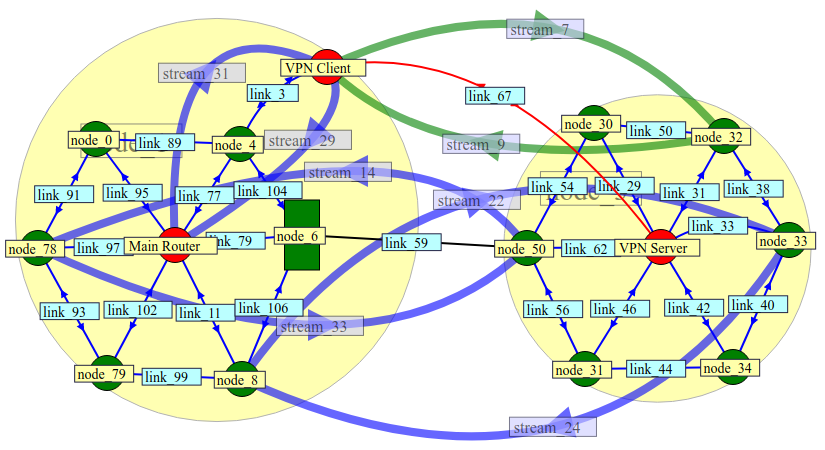
\includegraphics[width=6cm]{figures/vpn.png}
\caption{Two corporate networks }
\label{corporatenetwork}
\end{figure}

\begin{figure}
	\centering
		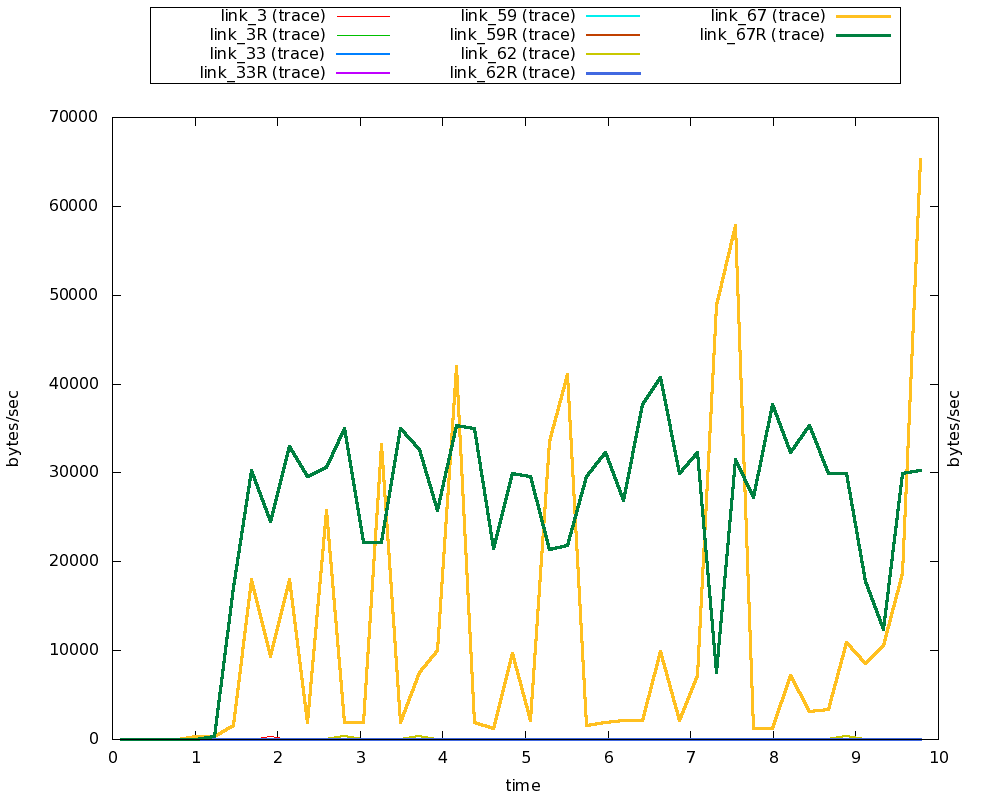
\includegraphics[width=6cm]{figures/vpn_traffic.png}
\caption{Traffic traces}
\label{Traffictraces}
\end{figure}

The Netml system provides services for analysis, design, and implementation
of networks \cite{addie2011netml}. These services are provided by means of a web
site Figure \ref{corporatenetwork}. No software is installed on users' computers (except in the form
of cached javascript). This system is used in teaching, by
computer science students, and in research into network analysis and design Figure  \ref{Traffictraces}. 
\iflonger
Most of the users of the Netml system, do not use it for an extended period of
time and therefore do not develop complex networks which incorporate a significant
investment. However, the security requirements of users of the system, and
its owners, are nevertheless important.
\fi

A key requirement of this system is that users can readily create their own
accounts and can reset their password if necessary when they have forgotten it.
Users can share networks that they create or load with each other, but by default
users cannot access the data of other users.

\subsection{Password Reset Service}
Many web systems include a service for allowing users to register,
authenticate, reset their password, and change personal details.
Password re-setting is one of the most common tasks faced by an
enterprise information help desk. Previous studies have shown that password
re-setting accounts for about one in four help desk requests \cite{bailey2014statistics}. The
human involvement in the password re-setting process is costly to
support. Thus, it is desirable to have an automated way to
authenticate a user for the purpose of password resetting in an
enterprise environment \cite{nimmy2014novel}. Reset mechanisms are therefore
essential at almost every password-protected site to handle forgotten
passwords. 

However, a password reset system is
complex to implement, and can easily include errors which open the system to attack
\iflonger
\cite{routh2018attacks,florencio2014administrator}. 
\else
\cite{routh2018attacks}. 
\fi

Typically, password reset systems make use of another system for checking
the credentials of a user to confirm the user's identity, for example,
the user's email system, or their phone. Any defect
in this second system (for example, if the user has revealed their email password
to another user, or has allowed others' free access to their phone) will compromise the password reset system
which relies on it, so the second system must be one with significantly
greater importance, for the user, for this type of design to be
satisfactory.\\

\subsection{Cross-site Script Attack Prevention}\label{cross-site-attack}

[Introduction to a method for preventing attacks based on grabbing
a session key and then attacking the server's account.]

The main strategy of xss is to exploit the vulnerability in the web application rather than to target these application's users. The attack will be by running maliciouse javascript code which inserted under the web page.

Although java script is a secure programming language, the improper implemntation and code bugs can exploited by XSS attack.
 XSS can allow the attacker to grab a session key, and then attacking the server's account and to perform actions on behalf of the user. \\

Section \ref{webservicessecurity} surveys current approaches to security design, including a description
of three specific approaches.
In Section \ref{initial} the original design of the Netml password reset system
is described; in Section \ref{expts}, a series of experiments in which this system
is attacked and then improved (a security audit), 
is described; in Section \ref{stakeholders}, 
a stakeholder security analysis is conducted and used to revise the design;
in Section \ref{proof}, the revised design is {\em proved}
to be correct (in respect of two of the rules). Conclusions are 
presented in Section \ref{concl}.

\section{Web Service Security Design}\label{webservicessecurity}
Because web services (including services provided via apps on mobile phones)
are a recent development and continue to evolve in both details and fundamentals,
principles of secure design of these services is also a new and evolving area of
research and development \iflonger\cite{AddieColman2010,Addie_Moffatt_Dekeyser_Colman2011}.
\else\cite{Addie_Moffatt_Dekeyser_Colman2011}.\fi

This section reviews three different approaches for securing web sites/services.
Each of these approaches is usually expressed as a completely independent
philosophy for achieving good security. We shall see that these approaches 
are actually complementary, and to achieve rigorous security all three approaches
are needed. Note that although we describe a design philosophy which is able, formally, to prove,
i.e.  guarantee, security, because no logical system can claim certainty in an absolute
sense (in mathematical logic, this fact is expressed in G\"odel's incompleteness theorem), the strategy 
of attacking the system remains useful, even after it has been
methodically proved to be correct.

The present paper does not apportion equal emphasis on all approaches
because the original contribution of this paper is 
in the third of them, together with the way the second approach joins
with the third to form a more comprehensive whole. The second approach
is the one summarised in Subsection \ref{audit} and applied
in Section \ref{expts}.
The third approach is summarised in Subsection \ref{stsecanal} and applied
to the Netml password reset system in Sections \ref{stakeholders} and \ref{proof}.


\subsection{Good Security Design Practice}
Good design takes security, ease of access, and usability into account,
striking a balance between protecting the system and ease of use. Good
practice has evolved a number of practical approaches like  minimizing
attack surface area \cite{bhardwaj2018reducing},  establish secure
defaults \cite{lai2018impact}, using the principle of defence in depth
\cite{toch2018privacy}, not trusting services \cite{ghirardello2018cyber},
keeping security simple \cite{thomsen2018network}, and fixing security
issues correctly \iflonger\cite {ali2018security, tabassum2018evaluating}.
\else \cite {tabassum2018evaluating}.\fi
These approaches  are used for  maintaining and improving security which
are so natural and important that they should be adopted as a first
layer of protection as a matter of standard practice, even when more
sophisticated approaches are also in use \cite {ross2018systems}.


\subsection{Security Auditing}\label{audit}

Strategies for breaking into web systems or services are under continuous
development by government and non-government organisations and individuals,
both those with friendly intentions and those who wish to exploit security
weaknesses for their own advantage. When
a new exploit is discovered, if it is discovered first by those with 
friendly intentions, defences against the exploit are usually developed
quickly and published. Exploits discovered by attackers with ill intent
can, of course, be deployed before web managers have the opportunity
to defend against them. Also, in the period of time immediately after
the defence against a new exploit has been published, there is still
an opportunity to attack web sites which have not deployed the newly developed
defences. This time can be somewhat extended due to the limitated expertise
of web-site owners and because the sequence of steps required to address a weakness
in a high-level framework can be quite lengthy.

A widely used strategy for improving web site or web service security is
to attempt to attack the site by using the strategies which are currently
known to be effective one-by-one, or simultaneously, to discover if the
site is vulnerable to any of these strategies. Since all of the strategies
tried are known, the defences against all of them are also almost certainly
known, and hence can be adopted by the web site.

Experiments of this type, and the resulting web service design improvements,
are described in Section \ref{expts}.

\subsection{Stakeholder Security Analysis}\label{stsecanal}

A more fundamental strategy which is not well-developed at present is
to seek to develop provably secure protocols and software for all aspects
of a web service \cite{whitman2011principles,mailloux2018examination,bishop2005introduction}.

The first step in this approach, which is developed further in 
Section \ref{stakeholders}, is to consider the point of view of all legitimate stakeholders
in relation to the service, and to enumerate a complete set of rules
required by each of these stakeholders, sufficient to ensure that they
will agree to actively participate in the service.
\subsubsection{Stakeholder Roles}\label{strol}
The roles are defined first, then their stakeholders, and access levels and features are set in those roles. Security rules are defined based on stakeholders roles, and not stakeholders themselves, where we can state the rule in terms of anyone who is playing a certain role. Stakeholder experiences should be shared to identify vulnerabilities that may occur while dealing with the service or part of the system under study. Most organizations consider the reputable more than the performance of their systems. Therefore, they adopt robust security solutions. However, access levels for sources as well as sensitive data often require additional restrictions above standard security requirements. Hence,  additional restrictions are identified and chosen with extreme care, ensuring their independence, and providing sources and data to the real interest without any other party who can access the current security restrictions.
\subsubsection{Stakeholder Business Rules}\label{stbsnrul}
Business rules refer to any rule relating to the way in which transactions are restricted. Business rules must be observed when designing and improving system security. In other words, even if the proposed security rules are enforced, they must be considered to be subject to the satisfactory standard by their professional organization. It is necessary to focus on Business rules  which are explicit rules on safety and try to study them and analyze them before drafting the security rules to avoid the contradiction.
The expectations of stakeholders which constitute a security case are considered mandatory and must be included in a security rule

\subsubsection{Stakeholder SWOT}\label{stswot}
The SWOT analysis tools are used to evaluate the security aspects for the stakeholders in the system Fig(). The first step is to determine the security objectives required by each stakeholders role and business rules within the specific service,Password Reset Service. And then identify the internal factors (strengths, weaknesses) and external factors (opportunities, threats) that are favourable and unfavourable to achieve those objectives.

Strengths are an opportunity to support security objectives, while weaknesses are considered to be the vulnerabilities that may impede the achievement of these objectives. The statement of the risks of weaknesses and the great efforts to fix them and clarify the strengths in the implementation of the security rules that prevent such circumstances are sufficient justification for obtaining the approval of the owners of the decision. On the other hand, the lack of funds and inconsistencies with business rules in achieving security objectives are weaknesses. In terms of opportunities, they are any initiatives available to support security objectives such as sources, expenditures, technologies, and security policies.Threats are related to the importance of the system and the sensitive information it contains. They often exploited weaknesses.

%These objectives support the protection of password reset service.
\subsubsection{Stakeholder Security Rules}\label{stsecrul}
\subsubsection{Assumption}\label{assmp} 
After completing security rules, assumptions are developed that simplify the logic necessary to complete the design process. The degree of simplification is determined depending on the sensitivity of the security issue. Security rules are therefore classified as optional or mandatory. Unlike the optional category, which is assumed or obvious assumptions, mandatory class assumptions are security requirements that need to be adopted in the design or development of system security.
\subsection{Stakeholder Security Design}\label{stsecdsgn} 
The main goal in the design phase is to know which of the mandatory security rules must be guaranteed and how to do it. When a particular  rule is not guaranteed directly,  this rule should be checked  that it follows from our assumptions and the rules which are enforced. However , there are three categories of rules: (i)assumptions; (ii) enforced rules; (iii)rules that must be proven, and through careful examining of the latter, the process of checking security becomes more reliable and systematic.

In addition, unrealistic assumptions may cause security vulnerability. Also, very strict assumptions can undermine security. However, the combination of the two methods can lead to simple and effective security design and achieve a higher security level in certain situations of critical importance.
\subsubsection{Inforcable Stakeholder Security Rules}\label{Instsecrul}
\subsubsection{Validation of Stakeholder Security Rules}\label{vlstsecrul}
\section{Original Design of Password Reset Service}\label{initial}

The original design of the password reset
service of the Netml system is described in Figures \ref{usersdl} and
\ref{seqdgnetmlorg}.
\begin{figure}
\begin{center}
\vspace{5mm}
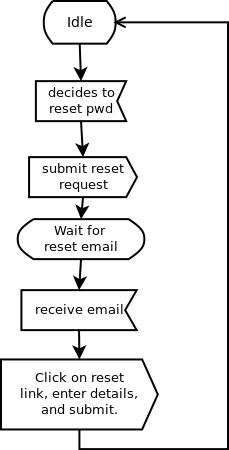
\includegraphics[width=37mm]{figures/resetpwd}
\caption{SDL diagram for User behaviour when resetting their password}
\label{usersdl}
\end{center}
\end{figure}

There is nothing exceptional about this design. However, in Section \ref{expts}
we discover that there are mistakes in the implementation of this design which
make it insecure.

\begin{figure}
	\centering
		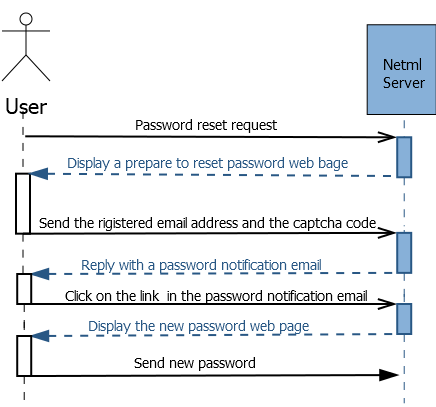
\includegraphics[width=5cm]{figures/User.png}
\caption{Sequence diagram for the Netml password reset  system }
\label{seqdgnetmlorg}
\end{figure}

\section{Break-in experiments}\label{expts}
\begin{figure}
	\centering
		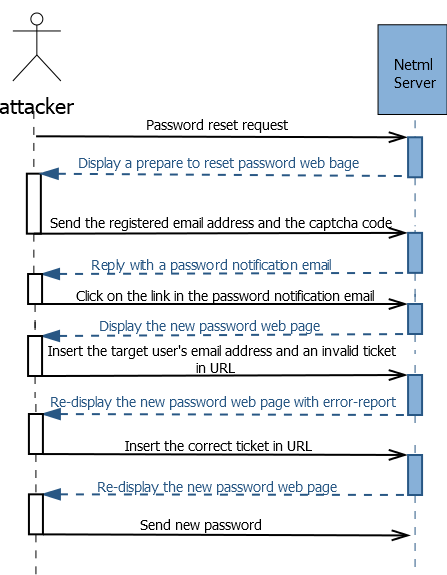
\includegraphics[width=6cm]{figures/attacker.png}
\caption{Sequence diagram for the Netml password reset  system under attack }
\label{seqdgnetmlattack}
\end{figure}
A series of experiments in which the system is attacked,
successfully, and then modified, are described in this section.
These experiments took the form described in Subsection \ref{audit},
i.e. a series of attacks were undertaken in accordance with known
vulnerabilities and observed behaviour of the system.

\subsection{First Experiment}
A detail not mentioned in Section \ref{initial} is that when an attempt
to update a user's password is made, with an invalid ticket, the web 
page which is prepared to report an error includes both the invalid
ticket, and the value that the ticket should have taken. This is a fatal
mistake (from the point of view of good security). There is no need
to report to an ordinary user what the value of the ticket should
have been. The reason this was included in the error-report web page
was to enable the software to be readily tested and debugged. However,
this information should have been removed from the error page
in the working system.

The procedure used to change the password of a different user was as
described in Figure \ref{seqdgnetmlattack}. First, the password reset system was used to reset the password
of the attacker (a perfectly valid procedure, with no ill intent or 
consequence). During this process, the URLs used at each stage
were observed. In particular, the URL which was used to complete
the reset of the password of user \verb|addie11| was of the form
shown in Listing \ref{registration}.
%???????
\iflonger\begin{listing}{\scriptsize
\begin{minted}[breaklines]{text}
https://netml.usq.edu.au/netml4_6/registration.jsp?
resetpwd=true&ticket=12345&uname=u1047621&fullName=fake&
email=u1047621@umail.usq.edu.au&organisation=USQ
\end{minted}
}
\caption{Form of URL which causes the password change web page to be displayed}
\label{registration}
\end{listing}\fi
%??????
A URL of this form was then used with the target user's email address and 
an invalid ticket. This generated an error report page which revealed
the value the ticket should have had. Finally, the correct ticket was
inserted into the URL and it was sent to the server. This URL caused
the web page for supplying a new password to be displayed, which was then
used to change the target user's password.

\subsection{Second Experiment}
After this defect was corrected, by removing the display of the valid
ticket in the error report web page, 
another experiment was carried out.
In some cases the algorithm used to generate tickets is known by attackers
because the source code for the server may be available or the attackers
may be able to guess the ticket algorithm
\cite{wang2018end}. In the revised Netml system, tickets were calculated as:
\begin{minted}[breaklines]{java}
hexsha(username+Calendar.getInstance()
.get(Calendar.DAY_OF_YEAR))
\end{minted}
In the present case this algorithm was deliberately revealed to the attacker.

In response to this attack, the ticket algorithm was changed to that 
shown in Listing \ref{ticketalg}. No attacks of the sort
described in this section were then able to succeed. A proof that
these type of attacks can't succeed is given in Section \ref{proof}.
% \section{The Revised Design}\label{designsec}  


	




